\section{Methods and Evaluation Protocol}
\subsection{Policy and editing interface}
Let $\pi_\theta(a_{t:t+H-1}\mid o_t,\ell,\xi_t)$ produce an action chunk from observation $o_t$, instruction $\ell$, and sampling seed $\xi_t$. Our target is the DROID joint-position checkpoint of $\policy$ \citep{pi2025pi05}: two $224\!\times\!224$ RGB views, seven joint positions, and a gripper state yield $H=15$ actions with eight used channels. RoboLab executes the chunks at 15\,Hz with a 900-step horizon. We evaluate only \textnormal{StackYellowOnRedTask}, with the fixed instruction ``Stack the yellow block on the red block''. Success uses the installed contact/geometry predicate; it does not additionally certify gripper release or sustained settling.

An editor $E_\phi$ proposes $\Delta_j$ from development evidence and prior feedback:
\begin{equation}
\tilde\theta_{j+1}=Q_{\rm bf16}\!\left[\theta_j+M_j\odot E_\phi(\theta_j,\mathcal D_{\rm dev},\mathcal H_j)\right].\label{eq:update}
\end{equation}
Here $M_j$ restricts entries, $Q$ applies deployment precision, and $\mathcal H_j$ records feedback. The gate accepts or reverts; editor weights $\phi$ remain fixed. Statistics, contrasts, projections, and tensor operations are permitted; optimization, regression fitting, policy-code/prompt changes, and training-derived task vectors are excluded. Gripper calibration is a separate runtime control.

We expose 18 action-expert down projections of shape $4096\times1024$. Each row maps one hidden-unit activation into the residual stream. A unit direction $v$ from a success/failure residual contrast can define $w'_i=w_i-\alpha\langle w_i,v\rangle v$, a direct operation rather than a fitted update. Interpretation depends on activation timing and later nonlinear computation; contrasts may reflect consequences rather than causes of failure.

\begin{figure}[t]
\centering
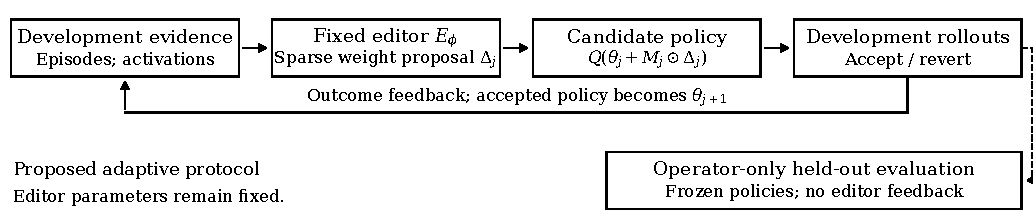
\includegraphics[width=\linewidth]{figures/edit_loop_paper.pdf}
\caption{Proposed enhancement loop. Development feedback can change the next proposal; held-out outcomes cannot. The large editor remains fixed while the smaller policy changes.}
\label{fig:loop}
\end{figure}

\subsection{Three research questions}
\textbf{RQ1: Can sparse repair improve outcomes?} Compare stacking edits with the base and gripper calibration; report success, nominal fixes/breakages, cost, and no-edit abstentions.

\textbf{RQ2: Does adaptive iteration help?} Compare three feedback-guided proposals with three base-anchored proposals committed before feedback. Evidence starts identically and budget caps match; feedback timing and usability differ. Retain all proposals and incumbents.

\textbf{RQ3: What behavior is preserved?} Count nominal fixes/breakages and repeat the base. This one-task study varies policy-sampling streams with environment seed zero; it tests neither new layouts nor cross-task preservation.

\subsection{Budget, controls, and analysis}
Four Astra (\textnormal{gpt-6-astra}, maximum effort) runs cross two restarts with two proposal modes. Each receives 32 common base episodes, 96 candidate episodes, 96 logical activation items, and two hours. Cumulative support is limited to 128 rows in two layers (131,072 entries); masks, deployed bfloat16 changes, norms, and hypotheses are recorded. 

\paragraph{Acceptance and attribution.}
For paired development outcomes $b_s,c_s\in\{0,1\}$, define nominal fixes $F=\sum_s(1-b_s)c_s$ and breakages $B=\sum_s b_s(1-c_s)$. Eligibility requires a deployed-value change, more successes than the base, and $B\leq2$. Rank eligible proposals by successes, smaller cumulative delta norm, then earlier order; otherwise retain the base. This engineering gate is not a non-inferiority test. Identity proposals consume evaluations but are ineligible. Accepted scores are nondecreasing by construction; retained points reuse observations.

Development and operator-only test slots are disjoint. A prospective v1.1 amendment precedes held-out outcomes and preserves discovery. Policies are grouped by actual bfloat16 values, checkpoint, runtime, task, prompt, environment settings, and threshold. Each unique edit, identity, and runtime control receives 64-base/64-candidate episodes; an extra 64-base repeat reuses the identity reference. Two-arm comparisons use ABBA32 order; global order is also fixed, not randomized. Round labels share estimates. Nominal pairing ensures neither equal observations nor variance reduction.

Report $\widehat\delta=(F-B)/n$ with nominal 95\% percentile intervals from 10,000 episode-slot bootstrap resamples, separately by restart. Wilson intervals are descriptive; uncorrected McNemar tests are exploratory. Shared 16-environment execution, reused streams, and selection limit independence. Two development blocks and two restarts cannot establish reliable cluster-adjusted inference or editor variability; no confirmatory significance, generalization, or non-inferiority is claimed.

Original budgets are 96 base/calibration, 384 candidate, and $320+128U$ final episodes for $U$ edited incumbents. Reserved blocks and failures remain charged; no silent retries or imputation.

\paragraph{Separate exploratory v2 follow-up.}
A separate pre-held-out protocol specifies three adaptive 32-episode proposals, 96 activation items, unchanged support/gate, a fresh 32-episode baseline, and disjoint test slots. Inference pads packets to 16; complete membership, positions, seeds, and outputs support replay without skips. Features widen bfloat16 to float32 (v1: float16); raw bits and padded costs remain recorded. Final scoring uses 128 episodes per unique incumbent or identity, with shared round labels. Searches freeze before held-out feedback; declared execution is v2 then v1.1, with ABBA32 comparisons. Changed execution, precision, and baseline preclude pooling or causal version rankings. Full protocols and hashes accompany the blog.

A model-neutral handoff supports optional matched Opus trials; none is reported. Policy-family and motor/perception comparisons are future extensions, outside these frozen RQs.
